% *********************************************************************
% © 2021–2026 Jeremy Sylvestre
%
% Permission is granted to copy, distribute and/or modify this document
% under the terms of the GNU Free Documentation License, Version 1.3 or
% any later version published by the Free Software Foundation; with no
% Invariant Sections, no Front-Cover Texts, and no Back-Cover Texts. A
% copy of the license is included in the appendix entitled “GNU Free
% Documentation License” that appears in the output document of this
% PreTeXt source code. All trademarks™ are the registered® marks of
% their respective owners.
%
% *********************************************************************

\newcommand*{\xmin}{-1}
\newcommand*{\xmax}{11}
\newcommand*{\ymin}{-0.5}
\newcommand*{\ymax}{1}

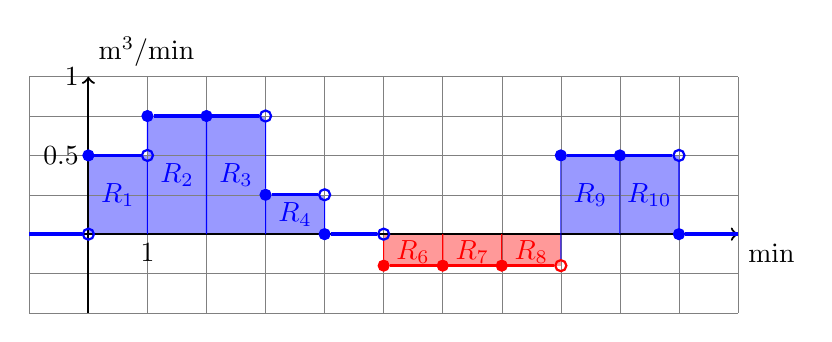
\begin{tikzpicture}
[
	closedpt/.style={circle,draw,fill,inner sep=0pt,minimum size=4pt},
	openpt/.style={circle,draw,inner sep=0pt,minimum size=4pt},
	xscale=0.75,
	yscale=2
]

	% rectangle fills
	\fill[blue!40!white] (0,0.5) rectangle (1,0);
	\fill[blue!40!white] (1,0.75) rectangle (3,0);
	\fill[blue!40!white] (3,0.25) rectangle (4,0);
	\fill[red!40!white] (5,-0.2) rectangle (8,0);
	\fill[blue!40!white] (8,0.5) rectangle (10,0);

	% grid
	\foreach \x in {-1,0,1,...,11} {
		\draw[very thin,gray] (\x,\ymin) -- (\x,\ymax);
	}
	\foreach \y in {-0.5,-0.25,0,0.25,...,1} {
		\draw[very thin,gray] (\xmin,\y) -- (\xmax,\y);
	}

	% label grid
	\foreach \x in {1} {
		\node[below] at (\x,0) {$\x$};
	}
	\foreach \y in {0.5,1} {
		\node[left] at (0,\y) {$\y$};
	}

	% axes
	\draw[->,thick] (\xmin,0) -- (\xmax,0) node[below right] {min};
	\draw[->,thick] (0,\ymin) -- (0,\ymax) node[above right] {$\mathrm{m}^3/\mathrm{min}$};

	% off
	\node[blue,thick,openpt] at (0,0) (stop) {};
	\draw[blue,very thick] (\xmin,0) -- (stop);

	% medium
	\node[blue,closedpt] at (0,0.5) (mstart) {};
	\node[blue,thick,openpt] at (1,0.5) (mstop) {};
	\draw[blue,very thick] (mstart) -- (mstop);

	% high
	\node[blue,closedpt] at (1,0.75) (hstart) {};
	\node[blue,thick,openpt] at (3,0.75) (hstop) {};
	\draw[blue,very thick] (hstart) -- (hstop);
	\node[blue,closedpt] at (2,0.75) (hmid) {};

	% area dividers
	\draw[blue,thin]
	  (hstart) -- (mstop)
	  (mstop) -- (1,0)
	  (hmid) -- (2,0)
	;

	% low
	\node[blue,closedpt] at (3,0.25) (lstart) {};
	\node[blue,thick,openpt] at (4,0.25) (lstop) {};
	\draw[blue,very thick] (lstart) -- (lstop);

	% area dividers
	\draw[blue,thin]
	  (hstop) -- (lstart)
	  (lstart) -- (3,0)
	;

	% off
	\node[blue,closedpt] at (4,0) (ostart) {};
	\node[blue,thick,openpt] at (5,0) (ostop) {};
	\draw[blue,very thick] (ostart) -- (ostop);

	% area dividers
	\draw[blue,thin]
	  (lstop) -- (ostart)
	;

	% leaking
	\node[red,closedpt] at (5,-0.2) (lstart) {};
	\node[red,thick,openpt] at (8,-0.2) (lstop) {};
	\draw[red,very thick] (lstart) -- (lstop);
	\node[red,closedpt] at (6,-0.2) (lmid1) {};
	\node[red,closedpt] at (7,-0.2) (lmid2) {};

	% area dividers
	\draw[red,thin]
	  (lstart) -- (ostop)
	  (lmid1) -- (6,0)
	  (lmid2) -- (7,0)
	;

	% medium
	\node[blue,closedpt] at (8,0.5) (mstart) {};
	\node[blue,thick,openpt] at (10,0.5) (mstop) {};
	\draw[blue,very thick] (mstart) -- (mstop);
	\node[blue,closedpt] at (9,0.5) (mmid) {};

	% area dividers
	\draw[blue,thin]
	  (mstart) -- (lstop)
	  (mmid) -- (9,0)
	;

	% off
	\node[blue,closedpt] at (10,0) (ostart) {};
	\draw[blue,very thick] (ostart) -- (\xmax,0);

	% area divider
	\draw[blue,thin]
	  (mstop) -- (ostart)
	;

	% rectangle labels
	\node[blue] at (0.5,0.25) {$R_1$};
	\node[blue] at (1.5,0.375) {$R_2$};
	\node[blue] at (2.5,0.375) {$R_3$};
	\node[blue] at (3.5,0.125) {$R_4$};
	\node[red] at (5.5,-0.115) {$R_6$};
	\node[red] at (6.5,-0.115) {$R_7$};
	\node[red] at (7.5,-0.115) {$R_8$};
	\node[blue] at (8.5,0.25) {$R_9$};
	\node[blue] at (9.5,0.25) {$R_{10}$};

\end{tikzpicture}
